%---------- Inleiding ---------------------------------------------------------
\documentclass{hogent-article}
\usepackage{tikz}
\usetikzlibrary{shapes.geometric, arrows}
\tikzstyle{startstop} = [rectangle, rounded corners, minimum width=3cm, minimum height=1cm,text centered, draw=black, fill=red!30]
\tikzstyle{io} = [trapezium, trapezium left angle=70, trapezium right angle=110, minimum width=3cm, minimum height=1cm, text centered, draw=black, fill=blue!30]
\tikzstyle{process} = [rectangle, minimum width=3cm, minimum height=1cm, text centered, draw=black, fill=orange!30]
\tikzstyle{decision} = [diamond, minimum width=3cm, minimum height=1cm, text centered, draw=black, fill=green!30]
\tikzstyle{arrow} = [thick,->,>=stealth]
\tikzstyle{process} = [rectangle, minimum width=3cm, minimum height=1cm, text centered, text width=3cm, draw=black, fill=orange!30]

\section{Introductie}%
\label{sec:introductie}

De toename van Artificiële Intelligentie (AI), Machine Learning (ML) en Deep Learning heeft geleid tot een groeiende vraag naar manieren om machine learning modellen op een schaalbare en efficiënte manier te implementeren en te beheren.
Binnen het vakgebied "AI \& Data Engineering" is er een cursus Machine Learning Operations, waar studenten leren van het opzetten van machine learning workspaces tot het monitoren van machine learning operations.
Dit onderzoek richt zich op een specifieke uitdaging binnen machine learning operations: Het lokaal draaien van machine learning pipelines.\newline

In deze context word er gebruik gemaakt van Azure ML pipelines, waarvan het onderliggende framework Kubeflow is. Kubeflow is een open-source machine learning toolkit op Kubernetes en zal centraal staan in dit onderzoek \autocite{Kubeflow2021}.
Er zal ook onderzoek worden gedaan naar alternatieven, die dan met elkaar worden vergeleken om eventueel een tweede Proof of Concept (PoC) op te stellen. hierbij zal gekeken worden naar hoe dat de verschillende frameworks en bibliotheken werken, welke programeertaal ze gebruiken en de verschillenede functies van elke framework.
Daarnaast worden de frameworks ook getest op de compatibiliteit van verschillende Operating Systems (OS). Deze test omvat gedetailleerde installaties van alle frameworks, waarvan de resultaten worden vastgelegd in een rapport.\newline

De focus ligt op het lokaal draaien van Kubeflow, een proces dat uitdagend is door de onduidelijke documentatie en de migratieproblemen van versie 1 naar versie 2.
Het onderzoek zal specifiek analyseren welke aspecten van de migratie problematisch zijn en waar de documentatie verbeterd kan worden.\newline

Dit onderzoek richt zich op IT-professionals die betrokken zijn bij Machine Learning Operations, specefiek voor de degenen die ML-pipelines lokaal willen draaien.
Het lokaal draaien van machinel learning pipelines met behulp van Kubeflow blijkt een uitdaging te zijn, vooral met betrekking tot de huidige migratieproblemen en gebrekkige documentatie.
De centrale probleemstelling is daarom: "Hoe kan een ML-pipeline lokaal worden uitgevoerd met behulp van een machine learning framework, rekeninghouden met de uitdagingen van de frameworks?"

%---------- Stand van zaken ---------------------------------------------------

\section{Literatuurstudie}%
\label{sec:state-of-the-art}

\subsection{Machine Learning}
Machine Learning (ML) is een onderliggend deel van Artificiële Intelligentie (AI), een snel groeiend vakgebied in het midden van informatica en statistiek, dat feit gebaseerde beslissingen in verschillende sectoren aanstuurt \autocite{Jordan2015}.
Door middel van het berekenen van wiskundige regels kan machine learning een verband leggen tussen gegevens om zo voorspellingen te genereren \autocite{Cybenko2001}.
Dit is mogelijk door het gebruik van machine learning algoritmen, hiermee kunnen computer leren van gegevens en hun prestatie in de loop van tijd verbeteren door middel van testen en validaties en zo nieuwe taken uit te voeren met nieuwe data \autocite{Shaveta2023}.
\subsection{CI/CD pipelines}
Een CI/CD (Continuous Integration/Continuous Deployment soms ook Continuous Delivery genoemd) zijn een cruciaal onderdeel van moderne softwareontwikkeling, voor het sneller en meer betrouwbare levering van web applicaties\\ \autocite{Singh2023}.
De effectiviteit van deze pipelines hangt sterk af van de juiste onderhoud en updates om in lijn te blijven met de veranderingen in systemen en technologiën \autocite{Zampetti2021}.
\subsection{Frameworks}
Een framework in programmeren is een herbruikbaar ontwerp, uitgedrukt als een reeks abstracte klassen en hun interacties \autocite{JuhaHautamaeki1997}. Het kan het softwareontwikkelingsproces verbeteren door ontwikkelaars in staat te stellen het gedrag ervan aan te passen aan hun huidige probleem \autocite{JuhaHautamaeki1997}. Frameworks kunnen worden gebruikt om dicipline in het programmeren te introduceren \autocite{PeiHsia1980}. Ze kunnen de kosten van het ontwikkelen van een toepassing verminderen door het hergebruik van zowel onterwerp als de code mogelijk te maken \autocite{DonRoberts2004}.
\subsection{Bibliotheken}
Programmeerbibliotheken zijn verzamelingen van vooraf geschreven code die hergebruikt kunnen worden om het ontwikkelproces te vereenvoudigen. Ze kunnen gebruik worden voor verschillende taken, zoals het ophalen van documenten, sorteren en indexeren \autocite{CharlesDavis1988}, en software ontwikkeling \autocite{Denert1979}.
\subsection{Kubeflow}
Kubeflow is een open-source platform met een collectie van machine learning tools biedt die compatiebel zijn met Kubernetes \autocite{Stein2020}. Het wordt vooral gebruik in DevOps-frameworks, waar het machine learning stacks en componenten zoals PyTorch en TensorFlow kan beheren \autocite{NGC2021}.
Kubeflow kan ook gebruik worden van end-to-end machine learning-oplossingen, waarbij pipeline-onderdelen de uitvoering van taken en het beheer van artefacten vergemakkelijken \autocite{Bisong2019}.

%Hier beschrijf je de \emph{state-of-the-art} rondom je gekozen onderzoeksdomein, d.w.z.\ een inleidende, doorlopende tekst over het onderzoeksdomein van je bachelorproef. Je steunt daarbij heel sterk op de professionele \emph{vakliteratuur}, en niet zozeer op populariserende teksten voor een breed publiek. Wat is de huidige stand van zaken in dit domein, en wat zijn nog eventuele open vragen (die misschien de aanleiding waren tot je onderzoeksvraag!)?

%Je mag de titel van deze sectie ook aanpassen (literatuurstudie, stand van zaken, enz.). Zijn er al gelijkaardige onderzoeken gevoerd? Wat concluderen ze? Wat is het verschil met jouw onderzoek?

%Verwijs bij elke introductie van een term of bewering over het domein naar de vakliteratuur, bijvoorbeeld~\autocite{Hykes2013}! Denk zeker goed na welke werken je refereert en waarom.

%Draag zorg voor correcte literatuurverwijzingen! Een bronvermelding hoort thuis \emph{binnen} de zin waar je je op die bron baseert, dus niet er buiten! Maak meteen een verwijzing als je gebruik maakt van een bron. Doe dit dus \emph{niet} aan het einde van een lange paragraaf. Baseer nooit teveel aansluitende tekst op eenzelfde bron.

%Als je informatie over bronnen verzamelt in JabRef, zorg er dan voor dat alle nodige info aanwezig is om de bron terug te vinden (zoals uitvoerig besproken in de lessen Research Methods).

% Voor literatuurverwijzingen zijn er twee belangrijke commando's:
% \autocite{KEY} => (Auteur, jaartal) Gebruik dit als de naam van de auteur
%   geen onderdeel is van de zin.
% \textcite{KEY} => Auteur (jaartal)  Gebruik dit als de auteursnaam wel een
%   functie heeft in de zin (bv. ``Uit onderzoek door Doll & Hill (1954) bleek
%   ...'')

%Je mag deze sectie nog verder onderverdelen in subsecties als dit de structuur van de tekst kan verduidelijken.

%---------- Methodologie ------------------------------------------------------
\section{Methodologie}%
\label{sec:methodologie}

Het ondezoek zal bestaan uit verschillende fasen. Er zal eerst een literatuurstudie worden uitgevoerd om inzicht te krijgen in de werking en
functies van verschillende frameworks en bibliotheken die machine learning pipelines ondersteunen.
Deze literatuurstudie zal gericht zijn op het vaststellen van mogelijke manieren om machine learning pipelines lokaal te draaien. Deze fase zal ongeveer 2 weken duren en gebruik maken van verschillende bronnen zoals online-artikelen en relevante rapporten om de nodige informatie te vinden. Als resultaat zal een sammenvatting geschreven worden met alle relevante informatie voor dit onderzoek.\\

In de volgende deze fase zullen volgende testen worden uitgevoerd op de Kubeflow and alternatieve frameworks en bibliotheken. De installatie word uitgevoerd en elke stap word beschreven en bekeken of er fouten komen. Daarnaast word er gekeken hoe dat machine learning pipelines lokaal draaien, hiervoor zal er een pipeline gemaakt worden die altijd de zelfde data verwerkt en bewerkingen uitvoert. deze data zal worden bijgehouden in een rapport.
Deze testen zullen op verschillende besturingssystemen worden uitgevoerd en met verschillende soorten data, hierdoor kunnen de resultaten goed worden geanalyseerd.\\

Na het verzamelen van de nodige data van de testen zal deze ook geanalyseerd worden. Dit zal gebeuren door de resultaten van de verschillende testen te vergelijken. Zo word gekeken hoe effectief de verschillende frameworks and bibliotheken de machine learning pipelines lokaal kan uitvoeren. Vervolgens wordt over de geanalyseerde data een conclusie geformuleerd.
Deze fase zal 6 weken duren.\\

Het uiteindelijke resultaat van dit onderzoek zal een volledig rapport zijn waarin de bevindingen en conclusies  gedetailleerd beschreven worden. Dit zal stapsgewijs gebeuren, waarin de belangerijkste bevindingen en conclusies worden aangetoond. Het rapport zal worden opgesteld met LaTeX. Dit zal 2 weken duren\\

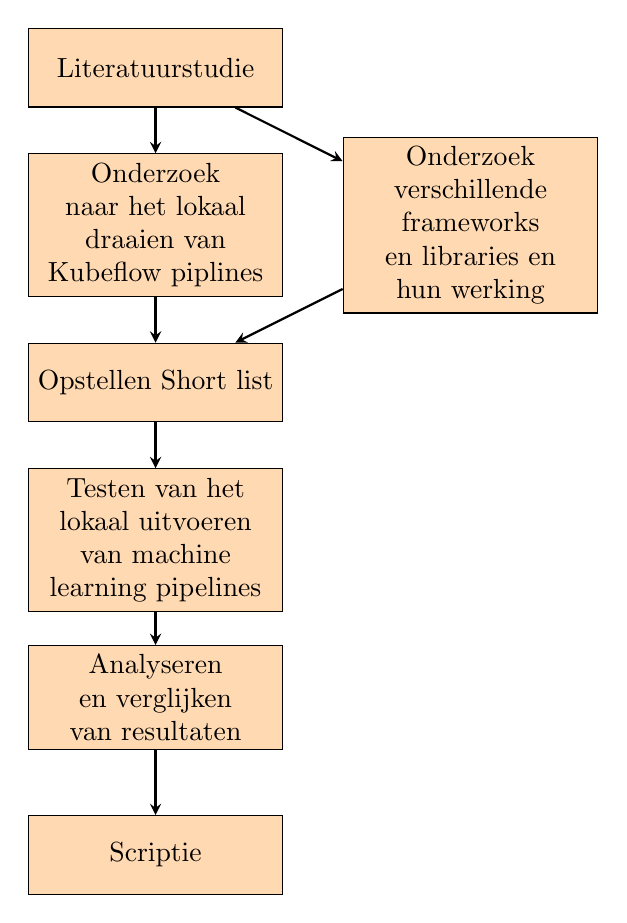
\begin{tikzpicture}[node distance=2cm]
  \node (pro0) [process] {Literatuurstudie};
  \node (pro1) [process, below of=pro0] {Onderzoek naar het lokaal draaien van Kubeflow piplines};
  \node (pro2) [process, right of=pro1, xshift=2cm] {Onderzoek verschillende frameworks en libraries en hun werking};
  \node (pro3) [process, below of=pro1] {Opstellen Short list};
  \node (pro4) [process, below of=pro3] {Testen van het lokaal uitvoeren van machine learning pipelines};
  \node (pro5) [process, below of=pro4] {Analyseren en verglijken van resultaten};
  \node (pro6) [process, below of=pro5] {Scriptie};
  \draw [arrow] (pro0) -- (pro1);
  \draw [arrow] (pro0) -- (pro2);
  \draw [arrow] (pro2) -- (pro3);
  \draw [arrow] (pro1) -- (pro3);
  \draw [arrow] (pro3) -- (pro4);
  \draw [arrow] (pro4) -- (pro5);
  \draw [arrow] (pro5) -- (pro6);
  \end{tikzpicture}
%Hier beschrijf je hoe je van plan bent het onderzoek te voeren. Welke onderzoekstechniek ga je toepassen om elk van je onderzoeksvragen te beantwoorden? Gebruik je hiervoor literatuurstudie, interviews met belanghebbenden (bv.~voor requirements-analyse), experimenten, simulaties, vergelijkende studie, risico-analyse, PoC, \ldots?

%Valt je onderwerp onder één van de typische soorten bachelorproeven die besproken zijn in de lessen Research Methods (bv.\ vergelijkende studie of risico-analyse)? Zorg er dan ook voor dat we duidelijk de verschillende stappen terug vinden die we verwachten in dit soort onderzoek!

%Vermijd onderzoekstechnieken die geen objectieve, meetbare resultaten kunnen opleveren. Enquêtes, bijvoorbeeld, zijn voor een bachelorproef informatica meestal \textbf{niet geschikt}. De antwoorden zijn eerder meningen dan feiten en in de praktijk blijkt het ook bijzonder moeilijk om voldoende respondenten te vinden. Studenten die een enquête willen voeren, hebben meestal ook geen goede definitie van de populatie, waardoor ook niet kan aangetoond worden dat eventuele resultaten representatief zijn.

%Uit dit onderdeel moet duidelijk naar voor komen dat je bachelorproef ook technisch voldoen\-de diepgang zal bevatten. Het zou niet kloppen als een bachelorproef informatica ook door bv.\ een student marketing zou kunnen uitgevoerd worden.

%Je beschrijft ook al welke tools (hardware, software, diensten, \ldots) je denkt hiervoor te gebruiken of te ontwikkelen.

%Probeer ook een tijdschatting te maken. Hoe lang zal je met elke fase van je onderzoek bezig zijn en wat zijn de concrete \emph{deliverables} in elke fase?

%---------- Verwachte resultaten ----------------------------------------------
\section{Verwacht resultaat, conclusie}%
\label{sec:verwachte_resultaten}
De data die zal verzameld worden van de testen zijn:
\begin{itemize}
  \item Hoe is de installatie of gebuik van de frameworks and bibliotheken verlopen?
  \item Hoelang duurde de installatie.
  \item Hoe word de zelfde pipeline uitgevoerd op de verschillende frameworks en bibliotheken.
  \item Hoelang duurde het uitvoeren van de pipelines op de verschillende frameworks en bibliotheken.
\end{itemize}

Er word verwacht dat er een duidelijk verschil zal zijn tussen de frameworks en bibliotheken. Kubeflow zal een uitdaging vormen door de onduidelijke documentatie, hierbij zal worden onderzocht of een ander alternatief mogelijk beter is.
Het uiteindelijke resultaat is een rapport die de resulaten zullen samenbrengen en conclusies trekt met betrekking tot de uitdaging van het lokaal draaien van draaien van Kubeflow, rekening houdend met de migratieproblemen en documentatiekwesties. Daarnaast zal het rapport aanbevelingen bevatten voor mogelijke verbeteringen in documentatie en migratieprocedures. Het rapport kan eventueel een beter alternatief bieden dan Kubeflow voor het lokaal draaien van machine learning pipelines, afhankelijk van de resultaten van de testen die gedaan werden.

%Hier beschrijf je welke resultaten je verwacht. Als je metingen en simulaties uitvoert, kan je hier al mock-ups maken van de grafieken samen met de verwachte conclusies. Benoem zeker al je assen en de onderdelen van de grafiek die je gaat gebruiken. Dit zorgt ervoor dat je concreet weet welk soort data je moet verzamelen en hoe je die moet meten.

%Wat heeft de doelgroep van je onderzoek aan het resultaat? Op welke manier zorgt jouw bachelorproef voor een meerwaarde?

%Hier beschrijf je wat je verwacht uit je onderzoek, met de motivatie waarom. Het is \textbf{niet} erg indien uit je onderzoek andere resultaten en conclusies vloeien dan dat je hier beschrijft: het is dan juist interessant om te onderzoeken waarom jouw hypothesen niet overeenkomen met de resultaten.